\documentclass[a4paper,12pt]{article}
% Resize margins:
\usepackage[top=1.5cm, bottom=2cm, left=3cm, right=2cm]{geometry}
\usepackage{natbib} % Citation package to cite by name (use plainnat
% bib style).
\usepackage{graphicx} % Graphics.
\usepackage[labelformat=simple]{subcaption} % Get subfigure environment.
\renewcommand\thesubfigure{(\alph{subfigure})} % Reference subfigures in parentheses.
\usepackage{empheq} % Loads mathtools, which in turn loads amsmath.
\usepackage{amssymb, accents, bm} % Maths (accents provide tilde under symbol).
\usepackage{hyperref} % Clickable links and table of contents.
\usepackage{siunitx} % SI unit package.
\usepackage{enumerate} % Labels of the 'enumerate' environment.
\graphicspath{{img/}} % Add a path to load images.
\usepackage{pgfplots} % Plots.
\pgfplotsset{width=7cm,compat=1.12} % Set size of all plots and assure 
% compatibility backwards.
\usepackage{todonotes} % Make to-do lists and visible comments.
\usepackage{tabularx, booktabs} % Tables, Commands to getter spacing above and 
% below the various rules in the table (\toprule, \bottomrule, \midrule, and 
% \cmidrule).
\usepackage{pgfplotstable} % plot x,y data from different files.
\usepackage{pdfpages} % Include external pdf.
\newcolumntype{Y}{>{\centering\arraybackslash}X} % Center content of the table, 
% stretching column(s) with specifier X to make table as wide as specified.

% Custom underline function:
\newcommand{\ubar}[1]{\mkern 1.5mu\underline{\mkern-1.5mu#1\mkern-1.5mu}\mkern 1.5mu}
% Double underline function:
\newcommand{\uubar}[1]{\ubar{\ubar{#1}}}
% Underline bold function:
\newcommand{\ubarbold}[1]{\ubar{\bm{#1}}}
% Double underline bold function:
\newcommand{\uubarbold}[1]{\uubar{\bm{#1}}}
% Undertlilde with bold face symbol:
\newcommand{\utilde}[1]{\underaccent{\sim}{\bm{#1}}}
% Double undertlilde with bold face symbol:
\newcommand{\uutilde}[1]{\underaccent{\approx}{\bm{#1}}}

\allowdisplaybreaks

\title{Computational Nonlinear Mechanics \\ \textbf{Assignment 2:\\
    Hyperelasticity and FE implementation of large strains}}

\author{Rostyslav Skrypnyk\footnote{Department of Mechanics and Maritime Sciences,
    rostyslav.skrypnyk@chalmers.se}}

\date{\today}

\begin{document}

\maketitle
\tableofcontents

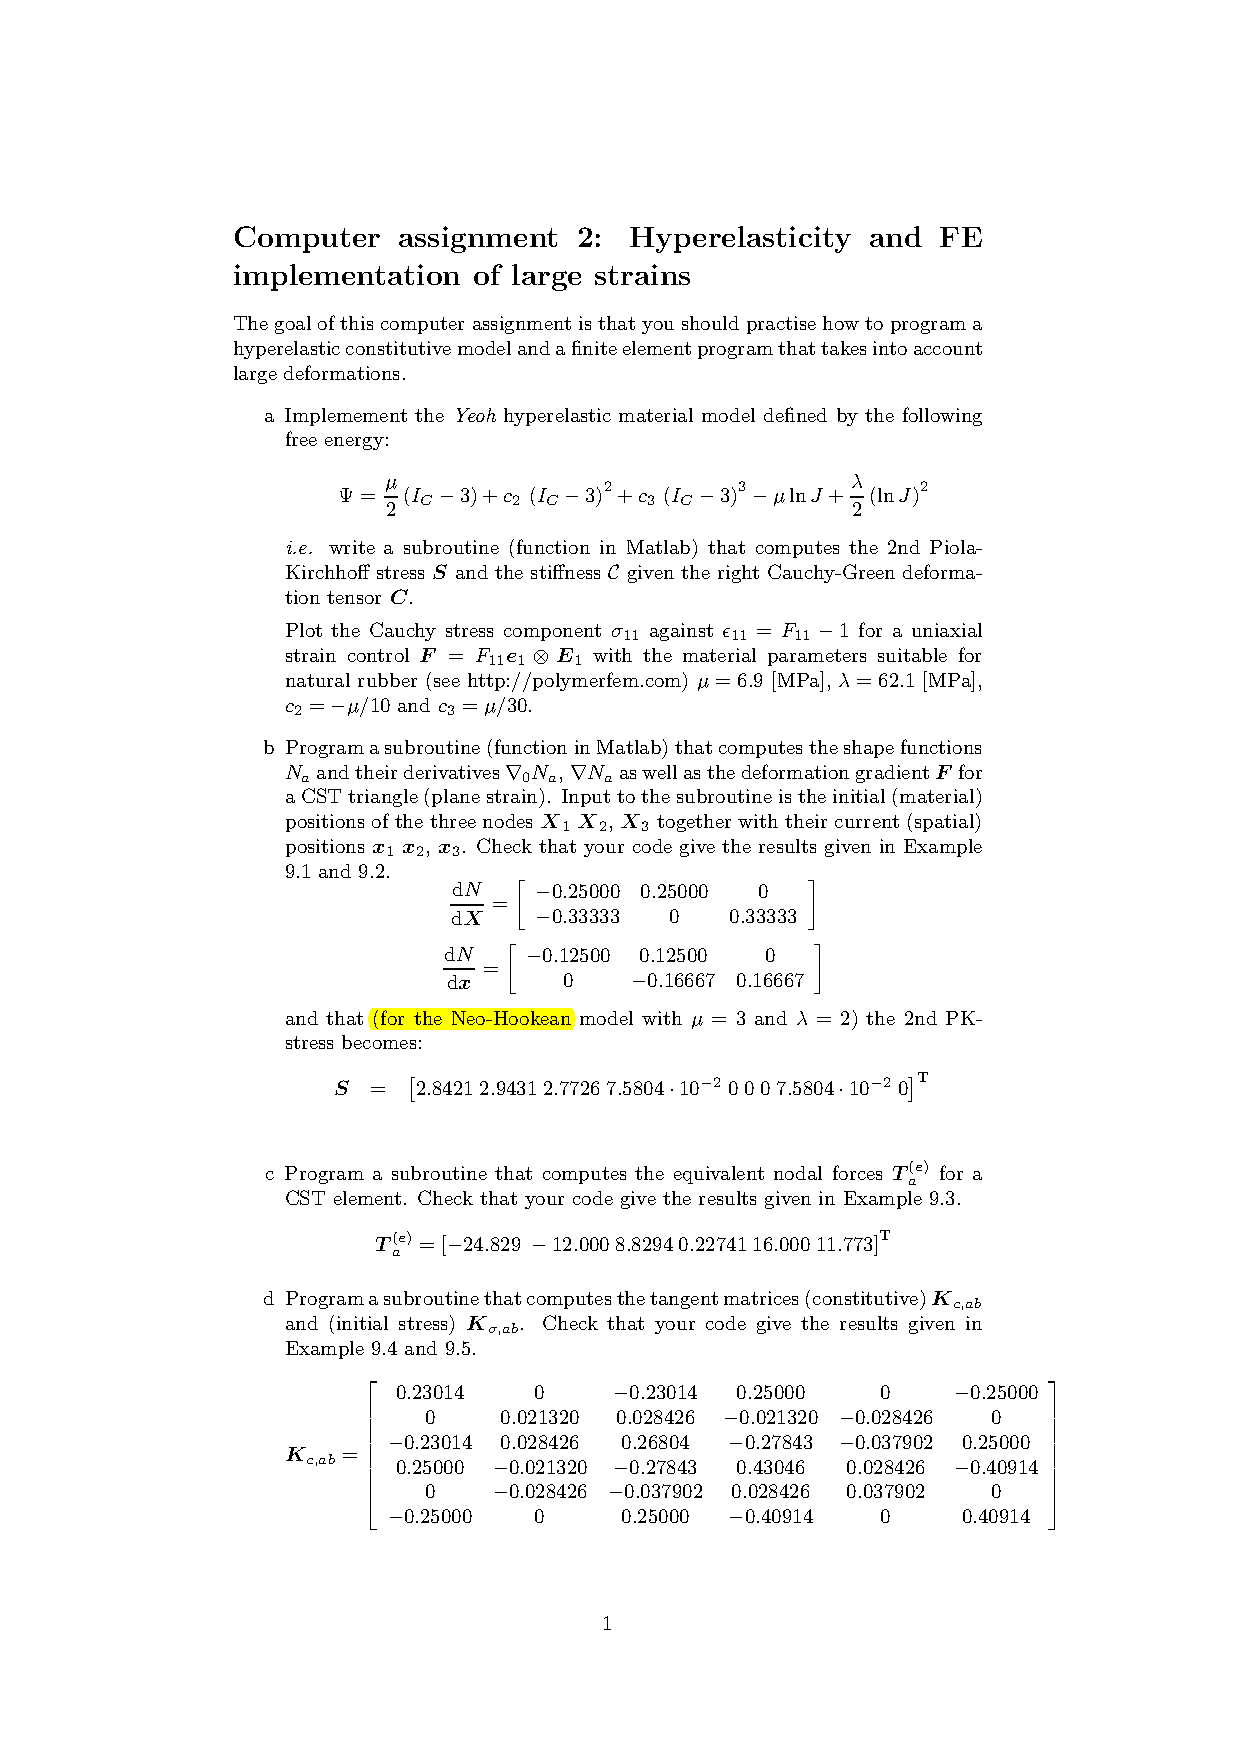
\includepdf[pages=-]{../CA2/CA2_MEkh.pdf} % Task description.
\clearpage
\section{Task A}
\label{sec:task-a}

The 2nd Piola-Kirchhoff stress can be obtained from free energy using
equation \eqref{eq:PK2} in \cite{Bonet2008}:
\begin{equation} \tag{6.18}
  \label{eq:PK2}
  \utilde{S} = 2 \frac{\partial \Psi}{\partial \utilde{C}} =
  2 \frac{\partial \Psi}{\partial I_{C}} \frac{\partial I_{C}}{\partial \utilde{C}} +
  2 \frac{\partial \Psi}{\partial II_{C}} \frac{\partial II_{C}}{\partial \utilde{C}}+
  2 \frac{\partial \Psi}{\partial III_{C}} \frac{\partial III_{C}}{\partial \utilde{C}}
\end{equation}
with derivatives of invariants of Green-Lagrange deformation tensor defined as
(\(J = \det \left( \utilde{F} \right)\))
\begin{align}
  \frac{\partial I_{C}}{\partial \utilde{C}} &= \utilde{I} \tag{6.19a} \\
  \frac{\partial II_{C}}{\partial \utilde{C}} &= 2 \utilde{C} \tag{6.19b} \\
  \frac{\partial III_{C}}{\partial \utilde{C}} &= J^{2} \utilde{C}^{-1} \tag{6.22}
\end{align}
Find the missing derivatives of the free energy (given in the task) with respect
to the invariants:
\begin{align}
  \frac{\partial \Psi}{\partial I_{C}} &= 
  \frac{\mu}{2} + 2 c_{2}\left( I_{C} - 3 \right) + 3c_{3}\left( I_{C} - 3 \right)^{2}\\
  \frac{\partial \Psi}{\partial II_{C}} &= 0 \\
  \frac{\partial \Psi}{\partial III_{C}} &= \frac{\lambda \ln{J} - \mu}{2 J^{2}}
\end{align}
Lastly, the expression for the 2nd Piola-Kirchhoff stress yields
\begin{equation}
  \label{eq:PK2yeoh}
  \utilde{S} = \left[ \mu + 4c_{2}\left( I_{C} - 3 \right) +
    6c_{3}\left( I_{C} - 3 \right)^{2}\right] \utilde{I} + 
  \left( \lambda \ln{J} - \mu \right) \utilde{C}^{-1}
\end{equation}
The Lagrangian elasticity tensor can be obtained using equation 
\eqref{eq:elast-tensor-Lagrange}:
\begin{equation} \tag{6.11}
  \label{eq:elast-tensor-Lagrange}
  \uutilde{C} = \frac{\partial \utilde{S}}{\partial \utilde{E}} = 
  2 \frac{\partial \utilde{S}}{\partial \utilde{C}}
\end{equation}
Expanding invariants to have explicit dependence on \(\utilde{C}\) yields
(\textit{note the overbar open product})
\begin{equation}
  \label{eq:dSdC}
  \frac{\partial \utilde{S}}{\partial \utilde{C}} = 
  \left[ 4c_{2} + 12c_{3}\left( I_{C} - 3 \right) \right] 
      \utilde{I} \otimes \utilde{I} + 
      \frac{\lambda}{2} \utilde{C}^{-1} \otimes \utilde{C}^{-1} +
      \left( \mu - \lambda \ln{J} \right) \utilde{C}^{-1} \overline{\otimes}
      \utilde{C}^{-1}
\end{equation}
Cauchy stress is a push-forward of the 2nd Piola-Kirchhoff:
\begin{equation} \tag{5.45b}
  \label{eq:cauchy-push}
  \utilde{\sigma} = J^{-1} \utilde{F} \cdot \utilde{S} \cdot \utilde{F}^{T}
\end{equation}
Figure~\ref{fig:sigma-eps} shows component of Cauchy stress plotted against
engineering strain for the situation of uniaxial strain control
\(\utilde{F} = F_{11} \ubar{\bm{e}}_{1} \otimes \ubar{\bm{E}}_{1}\).
It is evident that the curve is nonlinear.
\begin{figure}[th]
  \pgfplotstableset{
    create on use/Y/.style={create col/copy column from table={data/task_a_sig11.dat}{0}}
  }
  \centering
  \begin{tikzpicture}
    \begin{axis}[
      width = 0.95\textwidth,
      height=\axisdefaultheight,
%      tick label style={/pgf/number format/fixed},
      try min ticks=6,
      minor tick num=1,
      grid=both,
      xmin=0, xmax=1.5,
      xlabel = {\( \varepsilon_{11}\), [-]},
      ylabel = {\( \sigma_{11} \), [MPa]},
      ]
      \addplot table[y=Y,skip first n=1] {data/task_a_eps11.dat};
    \end{axis}
  \end{tikzpicture}  
  \caption{Cauchy stress component \(\sigma_{11}\) versus strain
    \(\varepsilon_{11} = F_{11} - 1\).}
  \label{fig:sigma-eps}
\end{figure}

The Matlab implementation of this task can be found in \texttt{yeoh.m}
(see section \ref{app:matlab-code}).

%%% Local Variables:
%%% mode: latex
%%% TeX-master: "../main"
%%% End:
 % \include uses pre- and post- \clearpage.
\section{Task B}
\label{sec:task-b}

For a constant strain triangle (CST) element, the shape functions can be defined as
\begin{equation}
  \label{eq:shape-func}
  N_{1} = 1 - \xi - \eta, \quad N_{2} = \xi, \quad N_{3} = \eta
\end{equation}

According to equations \eqref{eq:material-shape-grad}, the \textit{material}
gradient of shape function reads
\begin{equation} \tag{9.6ab} \label{eq:material-shape-grad}
  \ubar{\nabla}_{0}N_{a} = \frac{\partial N_{a}}{\partial \ubar{\bm{X}}} = 
  \left( \frac{\partial \ubar{\bm{X}}}{\partial \ubar{\bm{\xi}}} \right)^{-T}
  \frac{\partial N_{a}}{\partial \ubar{\bm{\xi}}} =
  \left( \frac{\partial \ubar{\bm{X}}}{\partial \ubar{\bm{\xi}}} \right)^{-T}
  \cdot \ubar{\nabla}_{\xi} N_{a}, \quad
  \frac{\partial \ubar{\bm{X}}}{\partial \ubar{\bm{\xi}}} 
  = \sum_{a=1}^{n} \ubar{\bm{X}}_{a} \otimes \ubar{\nabla}_{\xi}N_{a}
\end{equation}
%
\begin{equation}
  \ubar{\nabla}_{\xi} N_{a} = \left[
    \begin{array}{c}
      \dfrac{\partial N_{a}}{\partial \xi} \\
      \dfrac{\partial N_{a}}{\partial \eta} \\
	\end{array} \right] =
  \left[
    \begin{array}{c c c}
      \dfrac{\partial N_{1}}{\partial \xi} & \dfrac{\partial N_{2}}{\partial \xi} & \dfrac{\partial N_{3}}{\partial \xi}\\
      \dfrac{\partial N_{1}}{\partial \eta} & \dfrac{\partial N_{2}}{\partial \eta} & \dfrac{\partial N_{3}}{\partial \eta}\\
	\end{array} \right]  =
  \left[
    \begin{array}{c c c}
      -1 & 1 & 0 \\
      -1 & 0 & 1 \\
	\end{array} \right]
\end{equation}
Similarly, the \textit{spatial} shape function gradients are given as
\begin{equation} \tag{9.11ab}
  \label{eq:spatial-shape-grad}
  \ubar{\nabla} N_{a} = \frac{\partial N_{a}}{\partial \ubar{\bm{x}}} =
  \left( \frac{\partial \ubar{\bm{x}}}{\partial \ubar{\bm{\xi}}} \right)^{-T}
  \cdot \ubar{\nabla}_{\xi} N_{a}, \quad
  \frac{\partial \ubar{\bm{x}}}{\partial \ubar{\bm{\xi}}} 
  = \sum_{a=1}^{n} \ubar{\bm{x}}_{a} \otimes \ubar{\nabla}_{\xi}N_{a}
\end{equation}
Lastly, the deformation gradient can be expressed as
\begin{equation} \tag{9.5}
  \label{eq:deform-grad}
  \utilde{F} = \sum_{a=1}^{n} \ubar{\bm{x}}_{a} \otimes \ubar{\nabla}_{0} N_{a}
\end{equation}

The Matlab implementation of this task can be found in \texttt{shape\_gradients.m}
(see section \ref{app:matlab-code}).

%%% Local Variables:
%%% mode: latex
%%% TeX-master: "../main"
%%% End:
 
\section{Task C}
\label{sec:task-c}

The equivalent internal forces are given as
\begin{equation} \tag{9.15b}
  \label{eq:int-force}
  \ubar{\bm{T}}_{a}^{(e)} = \int_{v^{(e)}} \utilde{\sigma} \cdot \ubar{\nabla} N_{a}\, dv
\end{equation}
For a CST element of thickness \(t\) the same expression in local coordinates reads 
\begin{equation}
  \label{eq:int-force-local}
  \ubar{\bm{T}}_{a}^{(e)} = \int \int \utilde{\sigma} \cdot \ubar{\nabla} N_{a} \, t 
  \, dx \, dy =
  \int_{-1}^{1} \int_{-1}^{1} \utilde{\sigma} \cdot \ubar{\nabla} N_{a} \, t 
  \det \left( \frac{\partial \ubar{\bm{x}}}{\partial \ubar{\bm{\xi}}} \right) \,
  d\xi \, d\eta
\end{equation}
Apply Gaussian quadrature rule to compute the integral numerically:
\begin{equation}
  \label{eq:int-force-numer}
  \ubar{\bm{T}}_{a}^{(e)} \approx
  \sum_{i=1}^{\text{nip}} W_{i} \utilde{\sigma} \cdot \ubar{\nabla} N_{a} \, t 
  \det \left( \frac{\partial \ubar{\bm{x}}}{\partial \ubar{\bm{\xi}}} \right),
\end{equation}
where \(W_{i}\) is a weight for each of the integration points.
For a CST element, the number of integration points is 1 with coordinates
\(\xi = 1/3\), \(\eta = 1/3\) and the weight \(W = 0.5\).

The Matlab implementation of this task can be found in 
\texttt{get\_intern\_eq\_forces.m} (see section \ref{app:matlab-code}).

%%% Local Variables:
%%% mode: latex
%%% TeX-master: "../main"
%%% End:
 
\section{Task D}
\label{sec:task-d}

The \textit{constitutive} component of the tangent matrix relating node \(a\) to
node \(b\) is
\begin{equation} \tag{9.35}
  \label{eq:tang-mat-const}
  \left[ \uubar{\bm{K}}_{c,ab} \right]_{ij} =
  \int_{v^{(e)}} \sum_{k,l=1}^{3} \frac{\partial N_{a}}{\partial x_{k}}
  c_{ijkl} \frac{\partial N_{b}}{\partial x_{l}} \, dv, \quad i,j = 1,2,3
\end{equation}
The 4th order elasticity tensor in \textit{spatial} configuration can be computed
by pushing forward its counterpart in the \textit{material} configuration
\(\partial \utilde{S} / \partial \utilde{E}\):
\begin{equation}
  \label{eq:elast-tensor-Euler}
  \uutilde{c} = J^{-1} \utilde{F} \overline{\otimes} \utilde{F} \cdot
  \frac{\partial \utilde{S}}{\partial \utilde{E}} \cdot
    \utilde{F}^{T} \overline{\otimes} \utilde{F}^{T}
\end{equation}

For a CST element of thickness \(t\) equation \eqref{eq:tang-mat-const} can be
rewritten as
\begin{equation}
  \label{eq:tang-mat-const-CST}
  \uubar{\bm{K}}_{c,ab} \approx \sum_{i=1}^{\text{nip}} W_{i} \ubar{\nabla} N_{a}
  \cdot \uubar{\bm{D}} \cdot \ubar{\nabla} N_{b} t 
  \det \left( \frac{\partial \ubar{\bm{x}}}{\partial \ubar{\bm{\xi}}} \right),
\end{equation}
where \(\uutilde{c}\) was rearranged into matrix \(\uubar{\bm{D}}\) that
facilitates computations in the matrix form for 2D case:
\begin{equation}
  \label{eq:D-matrix}
  \uubar{\bm{D}} = \left[
    \begin{array}{c c c}
      c_{1111} & c_{1122} & c_{1112} \\
               & c_{2222} & c_{2212} \\
      \text{sym} &  & c_{1212}
	\end{array} \right] 
\end{equation}

The components of the \textit{initial stress} matrix are as follows:
\begin{equation} \tag{9.44c}
  \label{eq:tang-mat-init}
  \left[ \uubar{\bm{K}}_{\sigma,ab} \right]_{ij} =
  \int_{v^{(e)}} \sum_{k,l=1}^{3} \frac{\partial N_{a}}{\partial x_{k}}
  \sigma_{kl} \frac{\partial N_{b}}{\partial x_{l}} \delta_{ij} \, dv,
  \quad i,j = 1,2,3  
\end{equation}
Then for a CST element this becomes
\begin{equation}
  \label{eq:tang-mat-init-CST}
  \uubar{\bm{K}}_{\sigma,ab} \approx \sum_{i=1}^{\text{nip}} W_{i} \ubar{\nabla} N_{a}
  \cdot \utilde{\sigma} \cdot \ubar{\nabla} N_{b} \utilde{I} t 
  \det \left( \frac{\partial \ubar{\bm{x}}}{\partial \ubar{\bm{\xi}}} \right)
\end{equation}

The total tangent matrix is then
\begin{equation}
  \label{eq:tang-mat}
  \uubar{\bm{K}}_{ab} = \uubar{\bm{K}}_{c,ab} + \uubar{\bm{K}}_{\sigma,ab}
\end{equation}

The Matlab implementation of this task can be found in 
\texttt{get\_tangent\_matrices.m} (see section \ref{app:matlab-code}).

%%% Local Variables:
%%% mode: latex
%%% TeX-master: "../main"
%%% End:
 
\section{Task E}
\label{sec:task-e}

The given boundary value problem has been solved using Matlab script
\texttt{plate\_with\_hole.m} (see section \ref{app:matlab-code}).
Figure \ref{fig:bvp} shows total reaction force plotted against
displacement of the top nodes and the shape of the plate before
and after the deformation.
\begin{figure}[th]
  \centering
  % Reaction force
  \begin{subfigure}[t]{\textwidth}
    \begin{tikzpicture}
      \begin{axis}[
        width = 0.95\textwidth,
        height=\axisdefaultheight,
        minor tick num=1,
        grid=both,
        xlabel = {\(u_{x}\), [mm]},
        ylabel = {Reaction force, [N]},
        xmin=0, xmax=30
        ]
        \addplot table[skip first n=1] {data/force_displacement.dat};
      \end{axis}
    \end{tikzpicture}
    \caption{}
  \end{subfigure}

  % Geometry
  \begin{subfigure}[t]{\textwidth}
    \begin{tikzpicture}
      \begin{axis}[
        width = 0.95\textwidth,
        try min ticks=6,
        enlargelimits=false,
        axis equal image,
        axis on top,
        xlabel={\(x\), [mm]},
        ylabel={\(y\), [mm]}
        ]
        \addplot graphics[xmin=0,xmax=50,ymin=0,ymax=20] {mesh};
      \end{axis}
    \end{tikzpicture}  
    \caption{}
  \end{subfigure}
  \caption{(a) Reaction force versus displacement and (b) deformed mesh.}
  \label{fig:bvp}
\end{figure}

%%% Local Variables:
%%% mode: latex
%%% TeX-master: "../main"
%%% End:
 
\section{Matlab code}
\label{app:matlab-code}

The Matlab code can be found in the Git repository on
\href{https://github.com/iamrosk/hyperelasticity}{Github}.

%%% Local Variables:
%%% mode: latex
%%% TeX-master: "../main"
%%% End:


\bibliographystyle{abbrv}
\bibliography{references}

\end{document}

%%% Local Variables:
%%% mode: latex
%%% TeX-master: t
%%% End:
